\color{black}
\subsection{Specifica componenti View::Dialog}
\label{specificaDialog}
\begin{figure}[!h]

			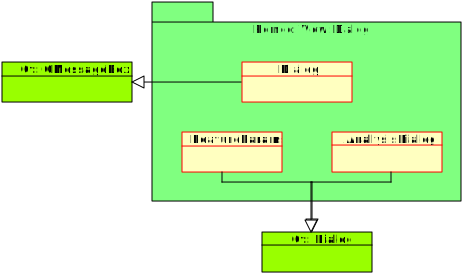
\includegraphics[width=0.7\linewidth]{../Specifica_Tecnica/Content/Immagini/Romeo__View__Dialog.png}
			\caption{Componente Romeo::View::Dialog}
			\label{comp_romeo::view::dialog}
\end{figure}
Componente che contiene tutte le classi che rappresentano le finestre di dialogo con cui l'utente potrà interagire
\pagebreak
%%%%%%%%%%%%%%%%%%%5
% 	DIALOG
%%%%%%%%%%%%%%%%%
\subsubsection{Dialog (class)}
\label{spedialog}
\begin{figure}[!h]
\centering
			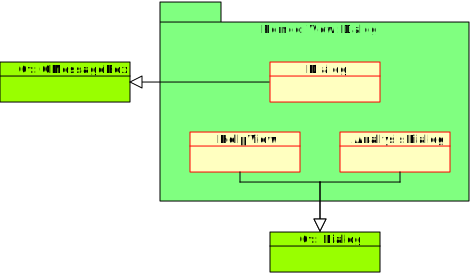
\includegraphics[width=1.1\linewidth]{./Content/Immagini/view/Dialog.png}
			\caption{Diagramma Classe Dialog: attributi e metodi}
			\label{cl_dia}
\end{figure}
\paragraph{Descrizione \\}
Classe che rappresenta le varie finestre di dialogo che mandano all'utente un messaggio, e che attende la pressione di un pulsante da parte dell'utente per proseguire. Possono essere messaggi che se accettati, interrompono la regolare operazione che era in esecuzione prima dell'apertura del messaggio di dialogo.
\paragraph{Utilizzo\\}
La classe viene utilizzata per dare messaggi all'utente.
\paragraph{Classi ereditate\\}
\begin{itemize}
\item Qt::QMessageBox.
\end{itemize}
%%%%%%%%%  METODI
\paragraph{\textcolor{black}{Metodi\\}}
\begin{itemize}
%costruttore
	\item \color{blue}\verb!- Dialog(title:QString\&, text:QString\&, info:QString\&, detail:QString\&, parent:QWidget*=0)!
\subparagraph*{Descrizione}
\color{black}Costruttore privato per la classe Dialog. Viene invocato dai metodi statici che mette a disposizione la classe in esame. \\
\subparagraph{Argomenti}
\begin{itemize}
\item \color{RoyalPurple} \verb!title: QString\\& !\\ title viene settato come titolo della finestra di dialogo;
\item \color{RoyalPurple} \verb!text: QString\\& !\\ text viene utilizzato per impostare il testo della finestra di dialogo;
\item \color{RoyalPurple} \verb!info: QString\& !\\ info viene utilizzato per impostare le informazioni della finestra di dialogo;
\item \color{RoyalPurple} \verb!detail: QString\& !\\ detail viene utilizzato per impostare i dettagli che la finestra di dialogo fornisce all'utente;
\item\color{RoyalPurple} \verb!parent: QWidget*=0 ! \\ Puntatore al QWidget padre di Dialog.
\end{itemize}
%dialogInfo
	\item \color{blue}\verb! + static dialogInfo(title:QString\&, text:QString\&, info:QString\&,! \\ \verb! detail:QString\&, parent:QWidget * = 0): int!
\color{black}
\subparagraph{Descrizione: }
Metodo statico che invoca la creazione di una finestra di dialogo che da un messaggio informativo. Ritorna il numero del pulsante che l'utente ha premuto. \\
\subparagraph{Note: }
\begin{itemize}
\item Questo metodo deve essere marcato statico.
\item Gli argomenti del metodo, vengono passati al costruttore della classe \emph{Dialog}.
\end{itemize}
%dialogCritical
\item \color{blue}\verb! + static dialogCritical(title:QString\&, text:QString\&, info:QString\&,! \\ \verb! detail:QString\&, parent:QWidget * = 0): int!
\color{black}
\subparagraph{Descrizione: }
Metodo statico che invoca la creazione di una finestra di dialogo che da un messaggio di criticità. Ritorna il numero del pulsante che l'utente ha premuto. \\
\subparagraph{Note:}
\begin{itemize}
\item Questo metodo deve essere marcato statico.
\item Gli argomenti del metodo, vengono passati al costruttore della classe \emph{Dialog}.
\end{itemize}
%dialogQuestion
\item \color{blue}\verb! + static dialogQuestion(title:QString\&, text:QString\&, info:QString\&,! \\ \verb! detail:QString\&, parent:QWidget * = 0): int!
\color{black}
\subparagraph{Descrizione: }
Metodo statico che invoca la creazione di una finestra di dialogo che richiede una risposta da parte dell'utente. Ritorna il numero del pulsante che l'utente ha premuto. \\
\subparagraph{Note:}
\begin{itemize}
\item Questo metodo deve essere marcato statico.
\item Gli argomenti del metodo, vengono passati al costruttore della classe \emph{Dialog}.
\end{itemize}
%DialogWarning
\item \color{blue}\verb! + static dialogCritical(title:QString\&, text:QString\&, info:QString\&,! \\ \verb! detail:QString\&, parent:QWidget * = 0): int!
\color{black}
\subparagraph{Descrizione: }
Metodo statico che invoca la creazione di una finestra di dialogo che da un messaggio di warning. Ritorna il numero del pulsante che l'utente ha premuto. \\
\subparagraph{Note:}
\begin{itemize}
\item Questo metodo deve essere marcato statico.
\item Gli argomenti del metodo, vengono passati al costruttore della classe \emph{Dialog}.
\end{itemize}
\end{itemize}
\pagebreak
%%%%%%%%%%%%%%%%%%
% 	featureParams
%%%%%%%%%%%%%%%%%%%%
\subsubsection{FeatureParams (class)}
\label{speFeaPar}
\begin{figure}[!h]
\centering
			\includegraphics[width=0.8\linewidth] {./Content/Immagini/view/FeatureParams.png}
			\caption{Diagramma Classe FeatureParams: attributi e metodi}
			\label{cl_fea}
\end{figure}
\paragraph{Descrizione \\}
Classe che rappresenta la finestra di dialogo che permette all'utente di impostare i valori dei parametri per una determinata Feature\g{}.
\paragraph{Utilizzo\\}
La classe viene utilizzata dalla finestra \emph{NewProtocolView} alla pressione del pulsante che permette l'inserimento di una nuova Feature\g{} nel \protocol in creazione. Dà la possibilità di impostare i valori dei parametri che richiede la Feature\g{}, dando comunque un valore di default per ogni parametro.
\paragraph{Classi ereditate\\}
\begin{itemize}
\item Qt::QDialog.
\end{itemize}

%%%%%%%%%%% ATTRIBUTI
\paragraph{\textcolor{black}{Attributi\\}}
\begin{itemize}
%FEATURES
\item \color{teal}\verb!-features: QVector<AFeature*>!
\color{black}
\subparagraph{Descrizione}
Contiene la lista di tutte le Feature\g{} rese disponibili da \project.
%params
\item \color{teal}\verb! - params:QStringList*!
\color{black} 
\subparagraph{Descrizione}
Lista contentente tutti i parametri richiesti dalla Feature\g{} che si vuole aggiungere.
%type
\item \color{teal}\verb! - type:QString!
\color{black} 
\subparagraph{Descrizione}
Stringa che contiene il tipo della Feature\g{} che si sta creando.

%feature

\item \color{teal}\verb! - feature: AFeature*!
\color{black} 
\subparagraph{Descrizione: }Puntatore polimorfo alla Feature\g{} selezionata.
%FeaturesComboBox
\item \color{teal}\verb! - featuresComboBox: ComboBox*!
\color{black} 
\subparagraph{Descrizione: }Visualizza le Feature\g{} contenute nel campo dati \emph{features}.
%firstWSize
\item \color{teal}\verb! - firstWSize: QLineEdit*!
\color{black} 
\subparagraph{Descrizione:} Linea di testo per impostare la dimensione della finestra per la Feature\g{} di primo ordine.

%secondWSize
\item \color{teal}\verb! - secondWSize: QLineEdit*!
\color{black} 
\subparagraph{Descrizione: }Linea di testo per impostare la dimensione della finestra per la Feature\g{} di secondo ordine.

%secondGlcm
\item \color{teal}\verb! - secondGlcm: QLineEdit*!
\color{black} 
\subparagraph{Descrizione:} Linea di testo per impostare il valore della GLCM\g{}.

%dynamicWSize
\item \color{teal}\verb! - dynamicWSize: QLineEdit*!
\color{black} 
\subparagraph{Descrizione: }Linea di testo per impostare la dimensione della finestra per la Feature\g{} di tipo dinamico.

%dynamicInitialFrame
\item \color{teal}\verb! - dynamicInitialFrame: QLineEdit*!
\color{black} 
\subparagraph{Descrizione: }Linea di testo per impostare il frame iniziale per la Feature\g{} dinamica.

%dynamicInitialFrame
\item \color{teal}\verb! - dynamicInitialFrame: QLineEdit*!
\color{black} 
\subparagraph{Descrizione:} Linea di testo per impostare il frame finale per la Feature\g{} dinamica.

%cancelButton
\item \color{teal}\verb! - cancelButton: QPushButton*!
\color{black} 
\subparagraph{Descrizione:} pulsante che permette all'utente di eliminare le modifiche fatte e non ancora salvate.

%okButton
\item \color{teal}\verb! - okButton: QPushButton*!
\color{black} 
\subparagraph{Descrizione:} pulsante che permette all'utente di confermare i dati inseriti e di conseguenza salvarli all'interno dell'applicativo \project{}.
\end{itemize}
%%%%%%%%%  METODI
\paragraph{\textcolor{black}{Metodi\\}}
\begin{itemize}
%costruttore
\item\color{blue}\verb!- FeatureParams(featureP: QVector<AFeature*>\&, parent:QWidget*=0)!

\subparagraph{Descrizione: }\color{black}Costruttore per la classe. \\
\subparagraph{Argomenti}
\begin{itemize}
\item\color{RoyalPurple} \verb! featureP: QVector<AFeature*>\& !\\ Vector di puntatori ad oggetti di tipo \emph{AFeature}. Utilizzato per inizializzare il campo dati \emph{features};
\item \color{RoyalPurple} \verb!parent: QWidget*=0 ! \\ Puntatore al QWidget padre di FeatureParams.
\end{itemize}
%setuplayout
\item\color{blue}\verb! -setupLayout(): void !
\color{black}
\subparagraph{Descrizione: }
 Metodo che ha il compito di impostare il layout del widget.

%setupObjectName
\item \color{blue}\verb! -setupObjectName():void!
\color{black} 
\subparagraph{Descrizione:} Metodo che ha il compito di impostare il nome di ogni oggetto, contenuto nel widget.

%addConnect
\item \color{blue}\verb! -addConnect(): void!
\color{black} 
\subparagraph{Descrizione: }Metodo che ha il compito di fissare tutte le istruzioni \emph{connect} degli oggetti che emetteranno un signal\g{} verso il rispettivo controller. 
%setupView
\item \color{blue}\verb! -setupView(): void !
\color{black} 
\subparagraph{Descrizione:} Metodo che ha il compito di impostare il layout del widget.

%createTop
\item \color{blue}\verb! -createTop():void!
\color{black} 
\subparagraph{Descrizione:} Metodo che ha il compito di creare la parte in alto della finestra di dialogo contenente i campi per l'inserimento dei valori dei parametri per la Feature\g{} selezionata.

%createLayout
\item \color{blue}\verb! -createLayout():void!

\color{black}
\subparagraph{Descrizione:} Metodo che ha il compito di creare il layout per la finestra di dialogo.
 
%createButtom
\item \color{blue}\verb! -createButtom():void!
\color{black}
\subparagraph{Descrizione:} Metodo che ha il compito di costruire la parte in basso del widget contenente il pulsante per il salvataggio dei valori inseriti oppure per poter reimpostare la form.

%createFeatureBox
\item \color{blue}\verb! -createFeatureBox():void!
\color{black}
\subparagraph{Descrizione: }Metodo che ha il compito di costruire il box contenente i campi per l'inserimento delle informazioni necessarie.

%createFirstBox
\item \color{blue}\verb! -createFirstBox():void!
\color{black}
\subparagraph{Descrizione: }Metodo che ha il compito di costruire il box contenente i campi per l'inserimento delle informazioni necessarie, relative alle Feature\g{} di primo ordine.

%createSecondBox
\item \color{blue}\verb! -createFirstBox():void!
\color{black}
\subparagraph{Descrizione:} Metodo che ha il compito di costruire il box contenente i campi per l'inserimento delle informazioni necessarie, relative alle Feature\g{} di secondo ordine.

%createDynamicBox
\item \color{blue}\verb! -createFirstBox():void!
\color{black}
\subparagraph{Descrizione:}
 Metodo che ha il compito di costruire il box contenente i campi per l'inserimento delle informazioni necessarie, relative alle Feature\g{} dinamiche.
 
%resetDefaulValues
\item \color{blue}\verb! -resetDefaultValues():void!
\color{black}
\subparagraph{Descrizione:}
 Metodo che ha il compito di impostare i campi di input ai valori di default.
 
%visibleBox
\item \color{blue}\verb! + visibleBox(type:QString\&): void!
\color{black}
\subparagraph{Descrizione:} Metodo che imposta la finestra di dialogo mostrando i campi corretti per l'inserimento dei valori dei parametri in base al valore della stringa passata come parametro al metodo.\\
\subparagraph{Argomenti:}
\begin{itemize}
\item \color{RoyalPurple} \verb! type: QString\& ! \\ rappresenta il tipo di Feature\g{} ovvero se di primo, secondo ordine o dinamica.
\end{itemize}

%resetBox
\item \color{blue}\verb! + resetBox(): void!
\color{black} 
\subparagraph{Descrizione:} Metodo che reimposta la finestra di dialogo, mostrando solamente il menu di selezione con le Feature{} disponibili.

%visibleBox
\item \color{blue}\verb! + visibleBox(type:QString\&): void!
\color{black}
\subparagraph{Descrizione:} Metodo che imposta la finestra di dialogo mostrando i campi corretti per l'inserimento dei valori dei parametri in base al valore della stringa passata come parametro al metodo.\\
\subparagraph{Argomenti}
\begin{itemize}
\item \color{RoyalPurple} \verb!type: QString\& ! \\ rappresenta il tipo di Feature\g{} ovvero se di primo, secondo ordine o dinamica.
\end{itemize}

%setFeature
\item \color{blue}\verb! + setFeature(featureF:AFeature*): void!
\color{black}
\subparagraph{Descrizione:} Metodo che imposta il campo dati \emph{feature}.\\
\subparagraph{Argomenti}
\begin{itemize}
\item \color{RoyalPurple} \verb!featureF: AFeature* !\\ puntatore polimorfo alla Feature\g{} selezionata il cui valore verrà dato al campo dati \emph{feature}.
\end{itemize}

%getFeatur
\item \color{blue}\verb! + getFeature(): AFeature*!
\color{black}
\subparagraph{Descrizione:} Metodo che ritorna un puntatore polimorfo alla Feature\g{} selezionata.\\

%featureSelected
\item \color{blue}\verb! + featureSelected(featureF:QString\&):void! (signal)
\color{black} 
\subparagraph{Descrizione:} Signal\g{} emesso quando l'utente seleziona una voce dal menu di selezione.
\subparagraph{Argomenti:}
\begin{itemize}
\item \color{RoyalPurple} \verb!featureF: QString\& !\\ identifica la selezione fatta dall'utente.
\end{itemize}

%ok
\item \color{blue}\verb! + ok(params:QStringList):void! (signal)
\color{black} 
\subparagraph{Descrizione:} Signal\g{} emesso quando dallo slot\g{} \emph{slotOk} quando i parametri inseriti hanno un valore corretto.
\subparagraph{Argomenti}
\begin{itemize}
\item \color{RoyalPurple} \verb!params: QStringList\& !\\ Lista contentente i valori di tutti i parametri settati dall'utente.
\end{itemize}

%slotOk
\item \color{blue}\verb!+ slotOk():void! (slot)
\color{black}
\subparagraph{Descrizione: }Slot\g{} che riceve il signal\g{} del click sul pulsante \emph{ok} della finestra di dialgo. Ha il compito di controllare se i valori inseriti per i parametri sono corretti e in caso, emette il signal\g{} \emph{ok}.\\ 
\end{itemize}
\color{black}
\pagebreak
%%%%%%%%%%%%%%%%%%%%%
% 	AnalysisDialog
%%%%%%%%%%%%%%%%%%%
\subsubsection{AnalysisDialog (class)}
\label{speAnaD}
\begin{figure}[!h]
\centering
			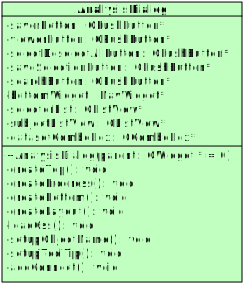
\includegraphics[width=0.6\linewidth] {./Content/Immagini/view/AnalysisDialog.png}
			\caption{Diagramma Classe AnalysisDialog: attributi e metodi}
			\label{cl_anaDia}
\end{figure}
\paragraph{Descrizione \\}
Classe che rappresenta la finestra di dialogo che viene visualizzata dall'utente durante l'esecuzione dell'analisi.
\paragraph{Utilizzo\\}
La classe viene creata quando l'utente ha scelto il dataset\g{} su cui eseguire l'analisi e le opzioni per la visualizzazione ed esportazione delle Feature\g{}. Mostra all'utente la barra di avanzamento dell'analisi; ad ogni Feature\g{} se precedentemente selezionato, verrà mostrato il risultato ottenuto dall'applicazione della Feature\g{} all'immagine associata al \subject{}. Mette inoltre a disposizione la possibilità di interrompere l'analisi, di proseguire senza più mostrare i risultati delle Feature\g{} oppure di proseguire con l'analisi con le impostazioni scelte.
\paragraph{Classi ereditate\\}
\begin{itemize}
\item Qt::QDialog.
\end{itemize}

\paragraph{\textcolor{black}{Attributi\\}}
\begin{itemize}
%nextButton
\item \color{teal}\verb!-nextButton: QPushButton*!
\color{black}
\subparagraph{Descrizione:} Pulsante che permette di proseguire l'analisi con le impostazioni scelte prima di inziare l'analisi.

%endButton
\item \color{teal}\verb! -previousButton:QPushButton*!
\color{black} 
\subparagraph{Descrizione:} Pulsante che permette di visualizzare l'immagine precedente a quella che si sta visualizzando al momento.

%progressBar
\item \color{teal}\verb! -progressBar:QProgressBar*!
\color{black} 
\subparagraph{Descrizione: }Identifica la barra di avanzamento che informa l'utente sul tempo mancante alla terminazione dell'analisi.

%cancelButton
\item \color{teal}\verb! -cancelButton: QPushButton*!
\color{black}
\subparagraph{Descrizione:} Pulsante che permette l'interruzione dell'analisi in corso.

%totalSub
\item \color{teal}\verb! -totalSubject: int!
\color{black}
\subparagraph{Descrizione:} Rappresenta il numero totale di Subject\g{} presenti all'interno del Dataset\g{} di cui si vuole far partire l'analisi.

%number
\item \color{teal}\verb! -number: int!
\color{black}
\subparagraph{Descrizione:} Rappresenta il numero di Subject\g{} su cui si vuole far partire l'analisi.

%currentSub
\item \color{teal}\verb! -currentSubject: int!
\color{black}
\subparagraph{Descrizione:} Rappresenta il numero del Subject\g{} attualmente processato.

%finished
\item \color{teal}\verb! -finished: bool!
\color{black}
\subparagraph{Descrizione:} Rappresenta un flag che vale true se e solo se l'analisi è stata completata.

%imageShow
\item \color{teal}\verb! -imageShow: int!
\color{black}
\subparagraph{Descrizione:} Rappresenta il numero di immagine che è visualizzata.

%images
\item \color{teal}\verb! -images: QVector<QImage*>!
\color{black}
\subparagraph{Descrizione:} Rappresenta la lista di immagini risultati dall'analisi.

%imagesDescription
\item \color{teal}\verb! -imagesDescription: QVector<QString>!
\color{black}
\subparagraph{Descrizione:} Rappresenta la lista delle informazioni delle immagini presenti all'interno di \textit{images}.
\end{itemize}

%%%%%%%%%%%%%%%%%%%% METODI
\paragraph{\textcolor{black}{Metodi\\}}
\begin{itemize}
%costruttore
\item \color{blue}\verb!- FeatureParams(featureP: QVector<AFeature*>\&, parent:QWidget*=0)!
\color{black}
\subparagraph{Descrizione:}
Costruttore per la classe. \\
\subparagraph{Argomenti:}
\begin{itemize}
\item \color{RoyalPurple} \verb!featureP: QVector<AFeature*>\& !\\ Vector di puntatori ad oggetti di tipo \emph{AFeature}. Utilizzato per inizializzare il campo dati \emph{features};
\item \color{RoyalPurple} \verb! parent: QWidget*=0  ! \\ Puntatore al QWidget padre di FeatureParams.
\end{itemize}

%updateButtonState
\item \color{blue}\verb! -updateButtonState(): void !
\color{black}
\subparagraph{Descrizione:} Metodo che ha il compito di aggiornare lo stato dei pulsanti sotto all'immagine che l'utente sta visualizzando.

%setupObjectName
\item \color{blue}\verb! -setupObjectName():void!
\color{black}
\subparagraph{Descrizione:} Metodo che ha il compito di impostare il nome di ogni oggetto, contenuto nel widget.
%showImage
\item \color{blue}\verb! -showImage(i : int):void!
\color{black} Metodo che ha il compito di visualizzare l'immagine che si trova all'indice rappresentato dal parametro passato al metodo.
\subparagraph{Argomenti:}
\begin{itemize}
\item \color{RoyalPurple} \verb! i: int! \\rappresenta il numero dell'immagine da far visualizzare nella view.
\end{itemize}

%addConnect
\item \color{blue}\verb! -addConnect(): void!
\color{black} 
\subparagraph{Descrizione:}
Metodo che ha il compito di fissare tutte le istruzioni \emph{connect} degli oggetti che emetteranno un signal\g{} verso il rispettivo controller.

%createProgress
\item \color{blue}\verb! -createProgress(): void !
\color{black} 
\subparagraph{Descrizione: }Metodo che ha il compito creare il layout contentente la barra di avanzamento dell'analisi.

%createTop
\item \color{blue}\verb! -createTop():void!
\color{black}
\subparagraph{Descrizione:} Metodo che ha il compito di creare la parte in alto della finestra di dialogo contenente la visualizzazione dell'anteprima dei risultati intermedi e la barra di avanzamento.

%createLayout
\item \color{blue}\verb! -createLayout():void!
\color{black} 
\subparagraph{Descrizione:} Metodo che ha il compito di creare il layout per la finestra di dialogo.

%createButtom
\item \color{blue}\verb! -createButtom():void!
\color{black}
\subparagraph{Descrizione:}
 Metodo che ha il compito di costruire la parte in basso del widget contenente i pulsanti per l'interazione con l'utente.

%closeEvent
\item \color{blue}\verb! #closeEvent(QCloseEvent* event):void!
\color{black}
\subparagraph{Descrizione:}
 Metodo virtuale che ridefinisce il comportamento del metodo presente nella classe \textit{Qt::QDialog}. Il metodo viene invocato quando Qt\g{} riceve una richiesta di chiusura di una finestra di più alto livello.
\subparagraph{Argomenti:}
\begin{itemize}
\item \color{RoyalPurple} \verb! event: QCloseEvent* ! \\Rappresenta l'evento con il quale il metodo verrà invocato; nel nostro caso riguarda un evento di chiusura della finestra.
\end{itemize}

%analysisfinish
\item \color{blue}\verb! +analysisFinish():void!
\color{black}
\subparagraph{Descrizione:}
 Metodo che ha il compito di aggiornare la view quando l'analisi è stata completata.
 
%setBarValue
\item \color{blue}\verb! +setBarValue(description: const QString\&):void!
\color{black}
\subparagraph{Descrizione:}
 Metodo che ha il compito di incrementare la barra di avanzamento e imposta il testo informativo.
\subparagraph{Argomenti:}
\begin{itemize}
\item \color{RoyalPurple} \verb! description: const QString\& ! \\ Rappresenta il testo informativo da far visualizzare all'utente nella barra di avanzamento.
\end{itemize}

%addImage
\item \color{blue}\verb! +addImage(image: QImage* ,description: const QString\&):void!
\color{black}
\subparagraph{Descrizione:}
 Metodo che ha il compito riceve l'immagine da mostrare nella finestra di dialogo.
\subparagraph{Argomenti:}
\begin{itemize}
\item \color{RoyalPurple} \verb! image: QImage* ! \\ Rappresenta l'immagine da visualizzare nella finestra di dialogo
\item \color{RoyalPurple} \verb! description: const QString\& ! \\ Rappresenta la descrizione dell'immagine passata come parametro.
\end{itemize}

%showPreviousImage
\item \color{blue}\verb! +showPreviousImage():void!
\color{black}
\subparagraph{Descrizione:}
 Metodo che ha il compito di visualizzare nella finestra di dialogo l'immagine precedente a quella attuale, se questa esiste.

%showNextImage
\item \color{blue}\verb! +showNextImage():void!
\color{black}
\subparagraph{Descrizione:}
 Metodo che ha il compito di visualizzare nella finestra di dialogo l'immagine successiva a quella attuale, se questa esiste.

%setImageDescr
\item \color{blue}\verb! +setImageDescription(txt: const QString\&):void!
\color{black}
\subparagraph{Descrizione:}
 Metodo che ha il compito di impostare la descrizione per la corrente immagine che si sta visualizzando.
\subparagraph{Argomenti:}
\begin{itemize}
\item \color{RoyalPurple} \verb! txt: const QString\& ! \\ Rappresenta il testo informativo relativa all'immagine corrente.
\end{itemize}

%incrementCurrentSub
\item \color{blue}\verb! +incrementCurrentSubject():void!
\color{black}
\subparagraph{Descrizione:}
 Metodo che ha il compito di incrementare il numero attuale di Subject\g{} presenti nella finestra di dialogo.
 
%nextImgage
\item \color{blue}\verb! +nextImage():void! (signal)
\color{black}
\subparagraph{Descrizione:} Signal\g{} emesso quando l'utente seleziona il pulsante next dalla finestra di dialogo.

%prevImgage
\item \color{blue}\verb! +previousImage():void! (signal)
\color{black}
\subparagraph{Descrizione:} Signal\g{} emesso quando l'utente seleziona il pulsante previous dalla finestra di dialogo.

%cancelAnalysis
\item \color{blue}\verb! +cancelAnalysis():void! (signal)
\color{black}
\subparagraph{Descrizione:} Signal\g{} emesso quando l'utente seleziona il pulsante cancel dalla finestra di dialogo.

%realclose
\item \color{blue}\verb! +realClose():void! (signal)
\color{black}
\subparagraph{Descrizione:} Signal\g{} emesso quando l'utente seleziona il pulsante yes dalla conferma di voler interrompere l'analisi.

%closeOnfinish
\item \color{blue}\verb! +nextImage():void! (signal)
\color{black}
\subparagraph{Descrizione:} Signal\g{} emesso quando l'analisi è stata completata.

\end{itemize}
\color{black}
\pagebreak